
\documentclass[a4j,titlepage]{ujarticle}
\usepackage[dvipdfmx]{graphicx}
\usepackage{enumerate}
\usepackage{url}
\usepackage{listings}


\title{
{課題提出型講義支援システム
\\
システム提案書}
\author{\\
\\
\\
\\
\\
Outing Corporation}
\date{\today}
}

\begin{document}
\maketitle


\tableofcontents

\clearpage

\section{はじめに}
% 課題提出型講義が今増えている
% 高知工科大学でもこういった講義がある
% その講義(実験)の概要
% 今の問題点
% その現状に対してのシステムの提案

% 情報系の学生の育成のために、課題を 〜〜 し、すぐさまフィードバックを受けることでなんとかかんとか こういった講義が増えている(根拠あればいいね)
%近年、情報システムの発展に伴い、課題をリアルタイムで提出すると言った講義が増えています。 % システム発展で他に
%その結果、課題提出型講義が大学の講義として増えているみたいなことを言いたい
%課題提出型の講義の一例として、高知工科大学の情報学群実験では、学生は各グループに分かれて、それぞれが与えられた課題に取り掛かります。
% そして、課題をこなすと、Teaching Assistant(以下TA)に、課題のチェックをしてもらい、
%合格するとそのグループは課題を終えることができます。(全然良い文章書けなかった)
%学生は、この課題チェックや質問を、挙手によって行うが、% 問題点述べて
%その結果、夜遅く(←ちょっと曖昧)まで課題が終わらないことが多々あります。
%このような現状に対して、課題チェックや質問を効率良く行うことができる、課題提出型講義支援システムをご提案いたします。

% 全然良い文章書けない〜〜〜

大学では、講義内容の理解度の確認や講義外での予習・復習を促すため、講義当日の提出を求める課題を提示する課題提出型の講義が開講されることが多々あります。
課題提出型の講義の一例として、高知工科大学様で開講される情報学群実験第1、情報学群実験第2が挙げられます。これらの講義では、学生は個人、または小数人で構成されたグループに分かれ、講義内で提示された課題に取り組みます。その後、課題達成の確認を高知工科大学様が雇用したTeaching Assistant(以下TA)に依頼し、TAにより正式に課題の達成が認められます。
現在、学生が課題の確認をTAに依頼する際、学生は挙手によって確認依頼の意を表明し、TAを自席に呼び、学生自身の課題の進捗の報告と課題の確認依頼を口頭で説明する必要があります。また、課題に対する質問をする場合も、課題の確認と同様の手順でTAに依頼をしなければなりません。

課題達成の確認と質問のどちらの場合も挙手制であることは、TA及び学生にとって非効率であると考えられます。
TAは学生の口頭説明により、初めて課題の確認か質問か、そして質問であればどの課題に対してどのような疑問があるのか、ということを知ることができます。
講義終了直前であれば、課題の確認や質問のために挙手をする学生が増えるため、TAは講義内に達成を義務付けられた通常課題を終えた学生に与えられる発展課題の確認や質問を求める学生への対応よりも、通常課題の確認や質問を求める学生への対応を優先したいという考えがあるため、学生の課題の進捗状況を事前に確認できないことが問題となります。挙手をする学生の人数によっては、TAは学生の課題の進捗状況を聞いてから対応を後に回す必要もあります。
加えて、どこで学生が挙手をしているのかを把握しがたいという問題があります。
また、TAはどのような質問がされるのかわからないため、質問によっては学生に話を聞いてから回答や対応を考える必要があると考えられます。課題の問題文に対する質問があれば、TAは教授に課題の仕様を確認する場合もあります。これら質問は同講義で既出の質問であり、同じ質問が複数の学生から上がることもあります。
以上の問題を含め、学生の課題の提出が講義時間内で終わらないことが多々あります。

このような現状に対して、課題達成の確認や質問を効率よく行うことができる、課題提出型講義支援システムをご提案いたします。

\section{解決できる経営課題}
現在、高知工科大学様で開講される課題提出型の講義では、学生の課題達成が講義時間内に終わらない状況にあります。
%高知工科大学で開講されている講義である情報学群実験では、講義時間以降も課題の提出が終わらない現状があります。 % 実験のこと知らない人に向けての説明をしたい
その背景として、以下のような課題が挙げられます。
\begin{enumerate}[(1)]
\item 課題の確認と質問が挙手制であり、挙手をしている学生の視認および把握が困難
\item 学生の挙手が同一の時間に集中した場合、どちらを優先すべきかわからない
\item 挙手に抵抗のある学生がいるため、挙手が同一の時間に集中する要因となっている
\item 質問に関しても同様に挙手制であり、課題の確認との区別ができない
\item TAは学生の課題の進捗状況が分からないため、講義終了前に学生の支援を行うことが困難
\end{enumerate}
%\begin{enumerate}[(1)]
%\item 課題の確認と質問が挙手制であり、TAが気づきにくい % なぜ気づきにくいかもう少し詳しくしたい あと「にくい」て言う言葉遣いがなんかもっといいの欲しい
%\item 挙手のタイミングが被り、どちらを優先すべきかわからない
%\item 質問に関しても同様に挙手制であり、課題のチェックとの区別ができない
%\item 挙手に抵抗のある学生がいる
%どう言った質問が来るのかが分かっていれば、TAも解決策を考えておけるみたいな
%\end{enumerate}
%それにより、TAの残業が深刻なものになっています。また、TAには時給が発生しており、学生の課題提出が終わらないことにより、
%大学側がTAに支払う金額も大きくなると考えられます。
講義時間内に学生の課題の提出が終わらないことにより、TAの講義時間外の就労が数時間に及ぶことがあります。TAには時給が発生しているため、受講している学生全員の課題提出が終わらない限り、高知工科大学様がTAにお支払いする金額も大きくなると考えられます。

 %こういった状況に対して学生側は授業中に課題の提出を終わらせることができず

\section{課題解決のための提案}
本提案書では前項で述べた課題を解決するものとして「課題提出型講義支援システム」を提案いたします。

\begin{enumerate}[(1)]
\item 学生からの課題の確認および質問のリクエストをまとめて可視化し、TAがスムーズに対応できる状況を提供します。
\item 学生からの質問は保存し、今後の講義に役立てることができます。
\item 各学生やグループの進捗状況を一覧で表示することで、TAが優先順位を考えて行動することができる状況を提供します。
\end{enumerate}

\section{課題解決のための方法}
前項で説明した提案につきまして、具体的な方法を説明いたします。
\begin{enumerate}[(1)]
\item 学生からの課題の確認および質問のリクエストをまとめ、課題の確認か質問のどちらをどの学生が行ったかを表示させる。
\item 学生からの質問は、データベースに蓄積させる。質問に対する回答を入力した場合は、質問は回答とともにデータベースに蓄積させることができる。TAは任意の折にデータベース上の質問と回答一覧を閲覧することができる。
\item 各学生やグループは課題の確認のリクエストとは別に、課題の進捗状況を選択し、送信する。
\end{enumerate}

%\begin{enumerate}[(1)]
%\item 各学生が状況を入力することで、TAが確認しやすい環境を作る %UIの作成 % UIとは
%\item 学生からの質問をデータベースに保存し、来年度それを参考にすることで %・・・ これはなんの課題なのか
%\item 各グループの進捗状況を入力し、TAがそれを監視することで、進捗が遅いグループにTAが時間を割くことができる。%そして全てのグループが講義時間内に課題を終わらせることができる状況を作る
%\end{enumerate}
\section{機能概要,前提条件,制約事項}

\subsection{機能概要}
\begin{enumerate}[(1)]
\item 学生が進捗状況を入力することで、TAが全体的な進み具合を把握することができます。
\item 学生がTAに、質問や課題の確認のリクエストを送ることができます。
\item 管理者は、グループ数や問題数を設定することができます。
\item 管理者は、過去の質問一覧を閲覧・編集することができます。 
\end{enumerate}

\subsection{前提条件}
\begin{enumerate}[(1)]
\item Raspberry Pi 3 がネットワークに接続できる環境で、このシステムを利用することが前提条件です。
\end{enumerate}

\subsection{制約事項}
\begin{enumerate}[(1)]
\item 管理者は、利用者のグループ数や課題の数を、あらかじめ入力することが必要です。
\end{enumerate}

%(1)管理者は課題の情報を入力することが必要である

\section{サービス利用までの流れ}
\subsection{人の流れ}
このシステムの利用者は、管理者側と実験を行う学生側の二者となります。
管理者は、講義が始まる前に、ネットワークに接続されているスマートフォンやパソコン等の端末から、システムの管理者画面にログインします。
そして、講義の課題について設定を行います。
学生側は、各グループの代表一人が、そのシステムにログインします。
そして、課題を行う中で進捗状況や質問を入力していきます。
管理者側は、入力された情報を確認し、実験を円滑に進めます。

システムの運用・保守については管理者が行い、質問等のデータベースの編集も行うことができます。
障害が発生した場合は、システムの再起動を行うことで前回更新した状況まで戻すことで対応します。 % 例えばどんな障害?システム自体の再起動かアプリだけの再起動か?
\begin{figure}[h]

\centering
   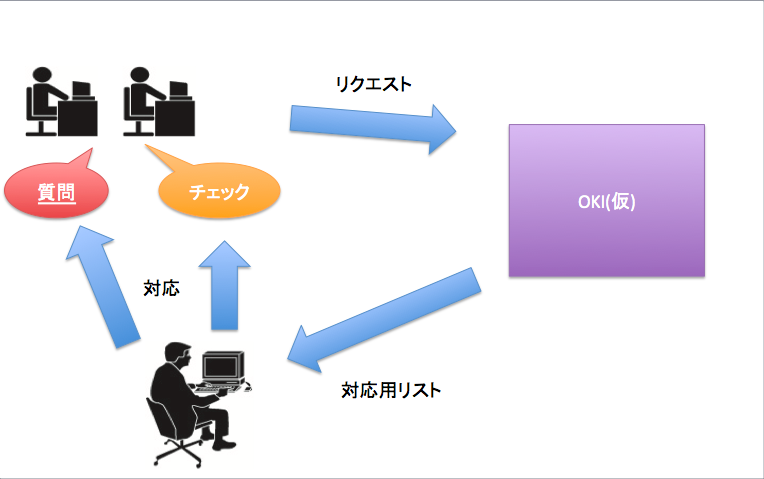
\includegraphics[width=13cm]{hito.png}
  \caption{主な流れ}
\end{figure}


\subsection{データの流れ}
このシステムは、ログイン画面によって管理者側と学生側の区別が行われます。そのため、システム自体は同様のものとなり、それとは別にサーバが % 学生側を利用者という言い方は良くない。ログイン画面で区別とは?システム自体が同様を別の言い方で
存在することでこのシステムの構成要素となります。
%システム内部での情報の流れは以下の図2のようになっています。 % どんな図作る?

サーバには学生側が登録の際に入力した個人情報や、質問の情報、課題の進捗状況などが格納されています。管理者は終了した講義の情報や次回の講義の
課題の情報を管理でき、利用者が前提条件に当てはまらなくなった場合には、登録の削除を行うことができます。
\begin{figure}[h]

\centering
   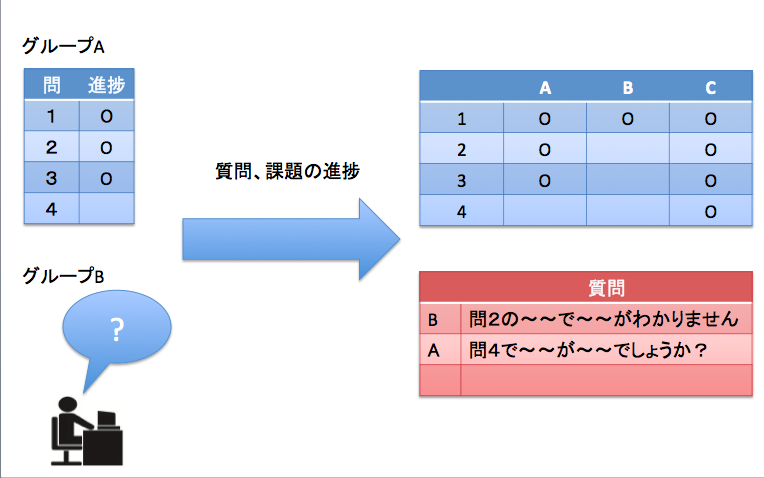
\includegraphics[width=13cm]{ui.png}
  \caption{データの集約の流れ}
\end{figure}

また、質問の一覧のデータを確認、削除することができ、そのデータベースの管理は管理者画面から行うことができます。

\section{想定する利用者}
このシステムが想定する利用者は、高知工科大学の教授、TA、学生となっています。 % もうちょっと詳しく。どんな学生かとか。利用者を別の言い方にしたい。

\section{導入・移行計画}
2018年2月1日をもってアプリケーションの公開を完了します。

\section{システムのハードウェア構成}
システムのハードウェア構成は、メインサーバとしての役割をはたす Raspberry Pi 3 が1台、そのシステムを操作するコンピュータ端末が1台となっています。 % システムを管理する端末って何?ソフトウェア構成が書かれてないが、ソフトウェア構成とは何?

\section{運用・保守}
提案システムの運用・保守については、全て管理者が行います。 % 管理者って誰?<ーTAや教授 これまでに上手いこと説明できてたっけ?

\section{作業標準}
システム開発にかかる作業標準は貴校ご指定のものを使用します。

\section{品質管理}
システム開発にかかる品質管理は貴校ご指定のものを使用します。

\section{工程計画}
工程計画は次の通りです。

外部設計完了:2017年11月27日

内部設計完了:2017年12月18日

開発完了:2018年1月25日

導入:2018年2月5日

\section{体制}
このシステムの開発は弊社システム部門の沖を中心として、7名のエンジニアにより実施します。

\section{システム化にかかる費用とその効果}
\subsection{費用}
システム化にかかる費用は以下の通りです。

% 表どうしよう。誰か計算して~
\begin{table}[htb]
  \begin{tabular}{|c|c|c|c|c|} \hline
    項目 & 単価(円) & 数量 & 金額(円) & 備考 \\ \hline
     Raspberry Pi 3 &  5000&  1&  5000& x \\ \hline
     システム開発人件費&  2000& 90日x7人x1.5時間&1890000&x  \\ \hline
     周辺機器&  10000&  1&  10000&  \\ \hline
      サーバー代&  10000&  5&  50000&5年使うと考えた場合  \\ \hline
    \multicolumn{3}{|c|}{合計}& 1955000円 &  \\ \hline
  \end{tabular}
\end{table}

%実験3c4cで平均残業時間が2時間で8人TAがいると考えると、合計672000の残業代がかかる。
%Raspberry Pi 3 が1台、周辺機器が1セット必要とすると、1万かかる
%そうすると、¥662000浮くはず で、開発人件費をどうするか
\subsection{効果}
効果の試算として、TAの授業後の平均残業時間が2時間とし、TAがその講義に8人ついていたとします。
現在のTAの時給は1,500円なので、1講義あたり8人 × 1,500円 × 2時間 で、1講義あたり24000円となります。
そして、1クォーターに同じ講義は14回程度あるので、 24,000円 × 14回となり、一つの講義で336,000円のコストが削減されます。
このシステムを活用する講義の例として情報学群実験を挙げていますが、情報学群実験は年間6講義あるので、 336,000円 × 6講義 = 2,016,000円が年間で
削減されます。% どれだけお金が浮くかを計算するよ

\section{本システム提案のアピールポイント}
%汎用性の高いシステムとなっているため、他の会議等での利用も可能です。
質問の内容が蓄積され、次年度の講義の改善へ繋げることができます。
Raspberry-pi 3 をサーバとして使用しているので、あらゆる場所で使用することができます。
場所を取らず比較的容易に導入できることで、導入、運用共に安価です。(文章要考察)


\section{用語の定義}
TA :「Teaching Assistant」の略称で、授業のアシストをする大学院生のこと。

管理者 : 教授やTAのこと。




\newpage

\end{document}
